\ylDisplay{Varras} % Ülesande nimi
{Siim Ainsaar} % Autor
{lõppvoor} % Voor
{2008} % Aasta
{G 9} % Ülesande nr.
{9} % Raskustase
{
% Teema: Staatika
\ifStatement
\begin{wrapfigure}[8]{r}{0.4\textwidth}
	\begin{center}
		\vspace{-25pt}
		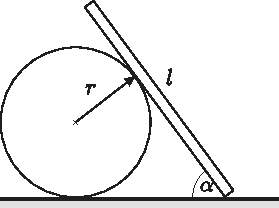
\includegraphics[width=\linewidth]{2008-v3g-09-yl}
	\end{center}
\end{wrapfigure}
Peenike homogeenne varras toetub ühe otsaga vastu põrandat (hõõrdetegur varda otsa ja põranda vahel on $\mu$) ning küljega vastu libedat horisontaalset silindrit (hõõrdetegur on tühiselt väike), vt joonist. Silinder on liikumatult kinnitatud põranda külge, varras on risti silindri teljega ning moodustab põrandaga nurga $\alpha$. Millise varda pikkuse $l$ korral jääb varras sellisesse asendisse püsima?
\fi


\ifHint
Pulgale mõjuvad neli erinevat jõudu: silindri ja pulga vaheline toereaktsioon, raskusjõud, maa ja pulga vaheline toereaktsioon ning hõõrdejõud. Pulga asend on stabiilne, kui jõudude ja jõumomentide tasakaalu tingimustest avaldatav hõõrdejõud ei ületa maksimaalset seisuhõõrdejõudu ning kui varda alaots ei tõuse õhku. Mõlemat tingimust väljendavad erinevad võrratused, mis peavad samaaegselt kehtima.
\fi


\ifSolution
\begin{center}
	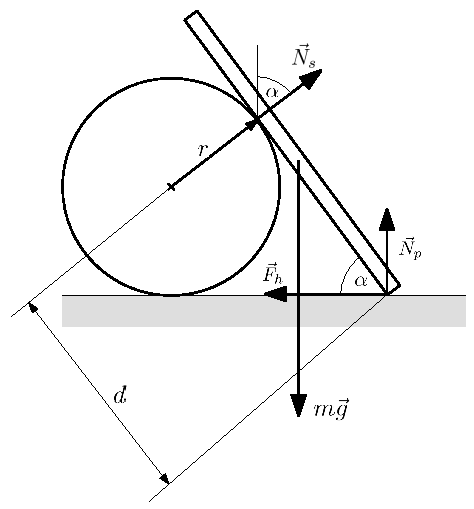
\includegraphics[width=0.7\linewidth]{2008-v3g-09-lah1.pdf}
\end{center}

Vardale mõjuvad põranda ja silindri toereaktsioonid (vastavalt $\vec N_p$ ja $\vec N_s$), hõõrdejõud $\vec F_h$ ja raskusjõud $m\vec g$ (vt ülemist joonist). Asend on stabiilne, kui jõudude ja jõumomentide tasakaalu tingimustest avaldatav hõõrdejõud ei ületa maksimaalset seisuhõõrdejõudu:
\begin{equation} \label{2008-v3g-09:eq1}
F_{h} \leq \mu N_{p}
\end{equation}
ja varda alaots ei tõuse õhku:
\begin{equation} \label{2008-v3g-09:eq2}
N_p \geq 0.
\end{equation}
Siin ja edaspidi võiksime sama hästi rangeid võrratusi kasutada, täpne libisemise piir on reaalselt saavutamatu.

Jõudude tasakaal horisontaalsihis:
\begin{equation} \label{2008-v3g-09:eq3}
F_h = N_s \sin \alpha
\end{equation}
ja varda sihis (võinuksime soovi korral valida ka muu sihi):
\begin{equation} \label{2008-v3g-09:eq4}
N_p \sin \alpha + F_h \cos \alpha = mg \sin \alpha.
\end{equation}
Olgu $d$ kaugus varda alaotsast toetuspunktini. Jõumomentide tasakaal varda alumise otsa suhtes annab (jällegi oleksid muud punktid võrdväärselt kasutatavad):
\begin{equation} \label{2008-v3g-09:eq5}
mg \frac{\ell}{2} \cos \alpha = N_sd.
\end{equation}
Avaldame jõud ja asendame võrratustesse:
\begin{align}
	(\ref{2008-v3g-09:eq5}),(\ref{2008-v3g-09:eq3}) & \Longrightarrow F_{h}=\frac{m g \ell}{2 d} \sin \alpha \cos \alpha, \label{2008-v3g-09:eq6}\\
	(\ref{2008-v3g-09:eq6}) \rightarrow(\ref{2008-v3g-09:eq4}) & \Longrightarrow N_{p}=m g\left(1-\frac{\ell}{2 d} \cos ^{2} \alpha\right),\label{2008-v3g-09:eq7} \\
	(\ref{2008-v3g-09:eq6}),(\ref{2008-v3g-09:eq7}) \rightarrow(\ref{2008-v3g-09:eq1}) & \Longrightarrow \frac{\ell}{2 \mu d} \sin \alpha \cos \alpha \leq 1-\frac{\ell}{2 d} \cos ^{2} \alpha \Longrightarrow\nonumber \\ 
	& \Longrightarrow \ell \leq \frac{2 \mu d}{\cos \alpha(\sin \alpha+\mu \cos \alpha)},\label{2008-v3g-09:eq8} \\
	(\ref{2008-v3g-09:eq7}) \rightarrow(\ref{2008-v3g-09:eq2}) & \Longrightarrow 1-\frac{\ell}{2 d} \cos ^{2} \alpha \geq 0 \Longrightarrow\nonumber \\ 
	& \Longrightarrow \ell \leq \frac{2 d}{\cos ^{2} \alpha}=\frac{2 \mu d}{\mu \cos ^{2} \alpha}. \label{2008-v3g-09:eq9}
\end{align}
(\ref{2008-v3g-09:eq9}) on leebem võrratus kui (\ref{2008-v3g-09:eq8}), mis on niisiis $\ell $ ülempiiriks (paremal nimetajas on selleks positiivne liige, $\sin \alpha$, juures). Kuna rangemat alampiiri ei ole, jääb selleks $d$.

$d$ leidmiseks ühendame varda alaotsa silindri teljega (joonis 2). Tekib kaks võrdset kolmnurka, millest:
\begin{equation}\label{2008-v3g-09:eq10}
d=\frac{r}{\tan \frac{\alpha}{2}}=\frac{r \sin \alpha}{1-\cos \alpha},
\end{equation}
\[
\begin{aligned}
(\ref{2008-v3g-09:eq10}) \rightarrow(\ref{2008-v3g-09:eq8}) \Longrightarrow \ell & \leq \frac{2 \mu r}{(\sin \alpha+\mu \cos \alpha) \cos \alpha \tan \frac{\alpha}{2}}=\\
&=\frac{2 \mu r}{(1+\mu \cot \alpha)(1-\cos \alpha) \cos \alpha} .
\end{aligned}
\]
Kokkuvõttes
\[
\frac{r \sin \alpha}{1-\cos \alpha} \leq \ell \leq \frac{2 \mu r}{(1+\mu \cot \alpha)(1-\cos \alpha) \cos \alpha}.
\]

\begin{center}
	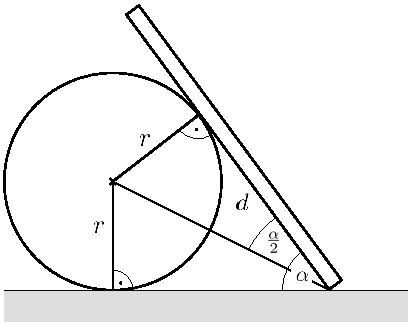
\includegraphics[width=0.7\linewidth]{2008-v3g-09-lah2}
\end{center}
\fi
}